% \begin{enumerate}
%     \item Physical phenomena
%     \begin{enumerate}
%         \item Elements involved (fluid and solid)
%         \item Properties of the elements that are meaningful for the problem
%         \item Observations or experimental knowledge $\rightarrow$ effects observed
%         \item New unseen problem $\rightarrow$ hypothesis of the effects to be observed
%     \end{enumerate}
    
%     \item Abstraction of the problem at hand and the physics
%     \begin{enumerate}
%         \item Equations for the physics studied (mechanics, thermal?, chemical?)
%         \item Mathematical model of the elements properties
%         \item Outer factors or conditions
%     \end{enumerate}
%     \item Analytical solution or numerical discretization.
%     \item Validation with experimental results
% \end{enumerate}

\graphicspath{{imgs/} {imgs/lam_turb} {imgs/spec}}

\section{Observations and empirical knowledge}

There are many examples of laminar and turbulent flows in nature that we are familiar with. In Fig.~\ref{fig:lam_turb} we show 3 examples, with water and flames. In the river image the water on the right side is laminar and on the left side it becomes turbulent. The calm flames of a candle rise initially in a laminar regime. On the bonfire example the flames are larger and show the different chaotic scale motions of a turbulent flow.

\begin{figure}[h!]
\centering
% \captionsetup{width=0.99 \textwidth}
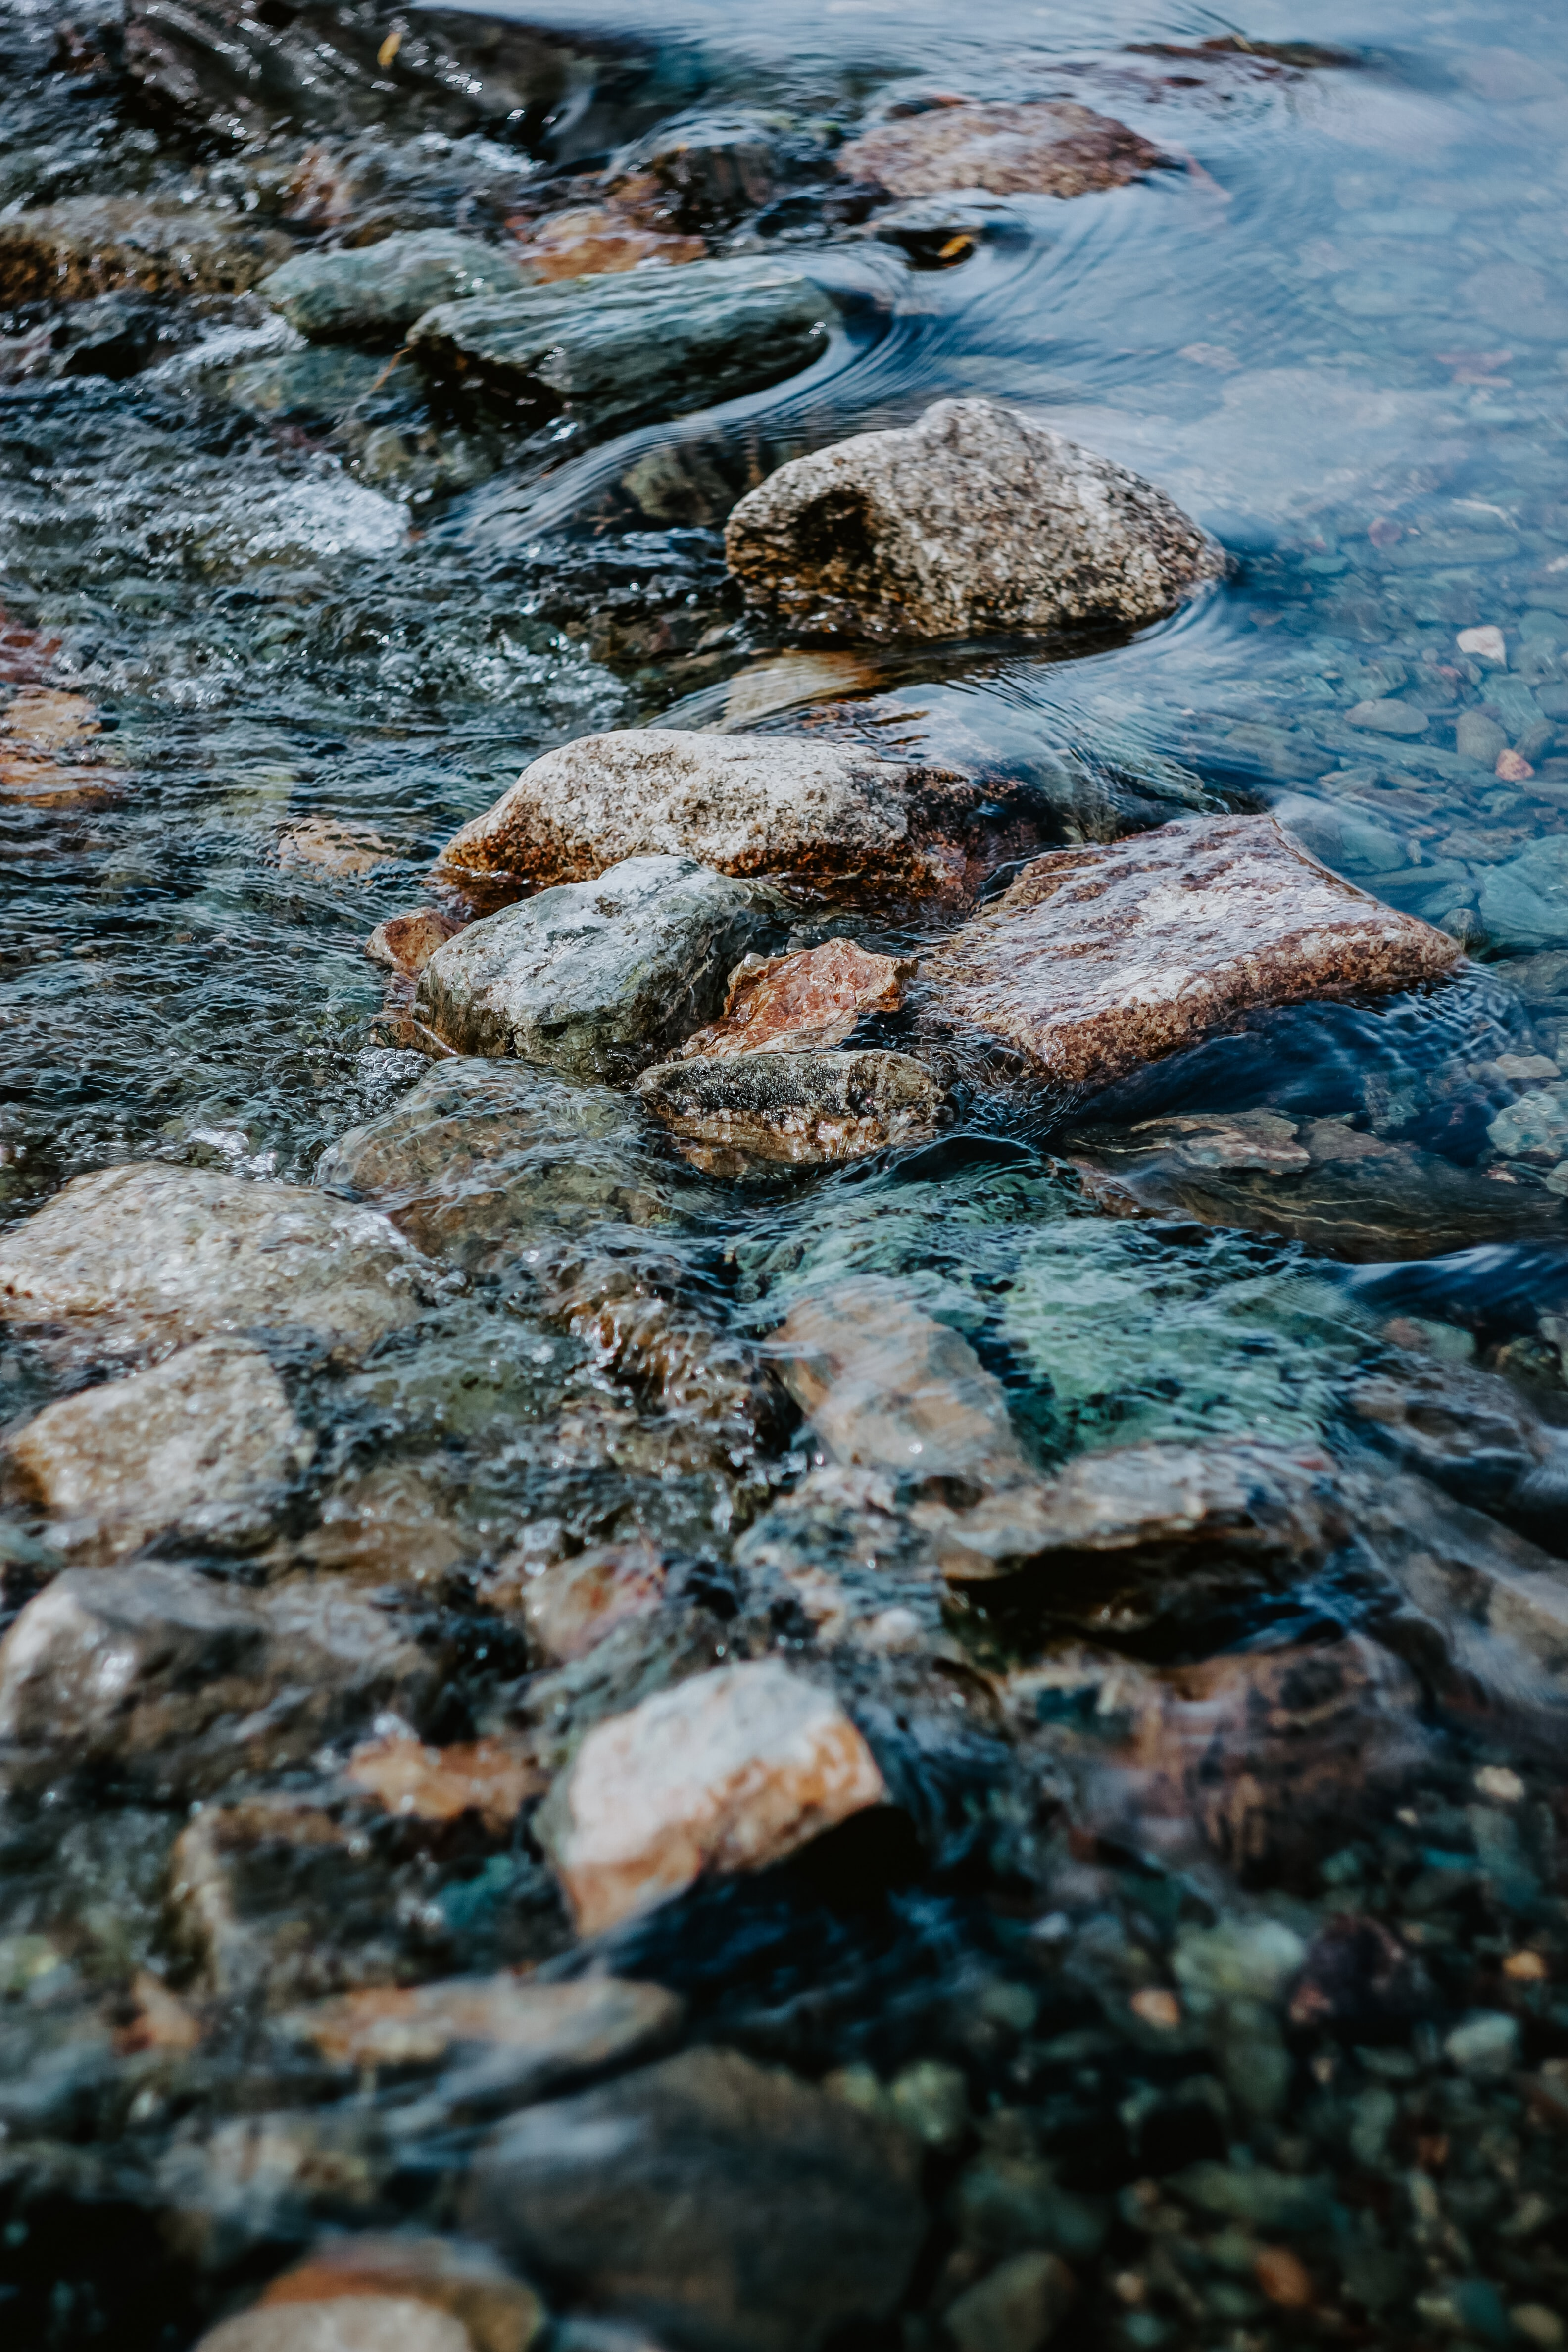
\includegraphics[height=5cm ]{laminar_turbulent_1.jpg}
% 
\includegraphics[width=5cm ]{llama_laminar.jpg}

\includegraphics[height=5cm ]{velas.jpg}
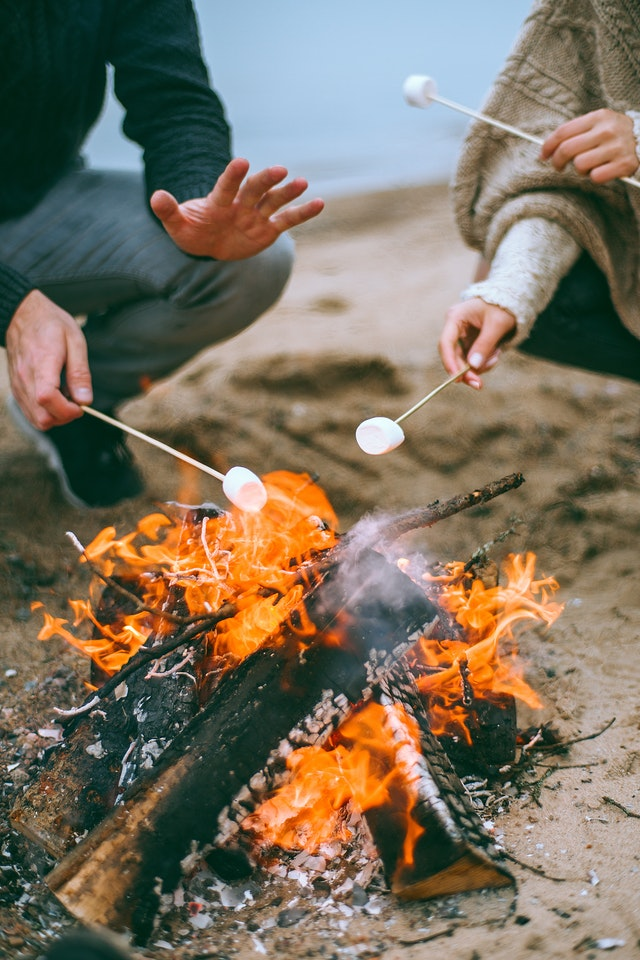
\includegraphics[height=5cm ]{llama_turb1.jpg}
\caption{ \label{fig:lam_turb} Examples of ordered laminar flow and chaotic turbulent motions in water and fire.
   }
\end{figure}

Laminar and turbulent regimes presents its advantages and disadvantages. 
In aerodynamic applications we usually focus in minimizing the friction produced at the solid wall-boundary or maximizing the lift/drag coefficient. In that aspect, the laminar boundary layer produces less friction than a turbulent boundary layer because it alters less the flow.
Detachment of the flow is an undesirable effect produced by strong adverse-pressure gradients, in this aspect, the laminar flow structure is more sensible to detachment under APG conditions than a turbulent flow.

To study turbulent boundary layers (TBLs) and the effects of adverse pressure gradients (APG) we will compare APG TBLs with a TBL subjected to zero pressure gradient (ZPG) conditions. The case of favourable pressure gradients (FPGs) stabilizes and relaminarizes the boundary layer, and its effects are not critical such as those provoked by APGs, where the boundary layer can detach from the wall producing undesirable effects such as an increase in drag or even to loose the aerodynamic controls in airplanes.
In order to study this kind of wall-attached fluid problem, first we should analyze the elements involved, such as the fluid and the solid elements.

\section{Fluid properties}

When studying the mechanics of a solid we track the positions, velocities and accelerations, forces and torques along its movement in space and time. This is the Lagrangian approach to mechanics.
For a flow of particles or a fluid it is more interesting to observe the flow variables at specific locations and observe the temporal change of those variables at those locations. This is the Eulerian approach that will be used to study the mechanics of a fluid flow. 

The main variables are the fluid velocities, $\vec{u}(\vec{x},t)=u_i=(u,v,w)$, and the pressure $p(\vec{x},t)$.
To simplify the study of adverse pressure gradient turbulent boundary layers the fluid analysed is isotropic (its properties are the same in all directions) and Newtonian, this implies that the viscous forces are a linear function of the strain rate tensor $s_{ij}=\pdv{u_i}/{x_j}$. As an example, the friction at the wall is $\tau_w=\mu \pdv{u}/{y}$
where $\mu$ is a constant factor, the dynamic viscosity.
The density and viscosity of the fluid combines into the kinematic viscosity $\nu=\mu/\rho$ with units $[m^2/s]$ independent of the mass. 
Since we consider the density and viscosity as constant and not affected by changes in temperature, the temperature of the fluid is not relevant and the energy and momentum evolution are decoupled.

\section{Solid properties}
In general, the solid boundaries are curved specially in aerodynamic applications where the curvatures are used to create differences in pressures that lead to forces in the desired directions. The forces in the direction of the inflow are called drag and the forces in the perpendicular direction is called lift. For curved boundaries, different coordinate systems are used. The local system of coordinates that changes with the solid boundary is where the surface forces are calculated. The surface forces are then projected onto the global coordinates associated with the inflow to obtain the lift and drag.
For flat plates with zero angle of attack the global and local coordinates are the same.
The surface of the flat plate that we study is rigid, and smooth, and no exchange of heat or mass is produced between the fluid and the solid. In the interface fluid/solid the only interaction is due to pressure and viscous forces that adapts the fluid velocity to the solid surface velocity.
The flat plate will be considered to be static in the global system of coordinates.


\section{Boundary layers}

Boundary layers are regions inside a fluid flow where certain features or changes in the properties of the fluid are concentrated. Historically the first idea of boundary layer is set for the adaptation region of the fluid momentum from outer conditions to the dynamical conditions in a solid surface.
Other boundary layers are for example thermal boundary layers where the focus is on the change of thermal properties.

When we consider the flow around a solid object in an incompressible regime, the flow can detect the presence of the solid object and adapt its trajectory. The flow then surrounds the solid starting from the leading edge and close to the solid surface the boundary layer is the region where the velocity of the flow adapts from the solid surface velocity to the outer flow velocity. The boundary layer thickness have to be defined according to the main idea of a region of the fluid close to the solid wall that encloses the major viscous effects created due to the fluid/surface interaction. An obvious effect of the presence of a wall is that the streamwise velocity has to adapt from the velocity of the solid boundary to the exterior velocity, commonly called velocity at the infinity $U_{\infty}$. 
In general, for a certain position of the wall, the velocity is measured in the wall-normal direction, obtaining a profile of streamwise velocities $u(y,t)$. Then $U_{\infty}=u(y\rightarrow \infty)$ is the unperturbed velocity and can change from one streamwise position to another.
In the case of zero-pressure gradient boundary layers, $U_{\infty}$ is taken as constant, since in a steady flow in the absence of viscous forces, $\pdv{u}/{x}$ should be zero. 

Since an obvious indicator of the boundary layer is the adaptation of the streamwise velocity, the boundary layer can be defined using this property and the $99\%$ thickness $\delta_{99}$ is defined as the wall-normal position where $u(y=\delta_{99}) = U_{\infty}$.
In Fig.~\ref{fig:lam_turb_profiles} we show an example on how the mean streamwise velocity $U(y)$ adapts from the velocity at the wall $u(y=0)=0$, to the outer velocity $U_{\infty}$, which has been scaled to be equal to 1, on a laminar and a TBL ZPG profiles.

\begin{figure}[h!]
\centering
% \captionsetup{width=0.99 \textwidth}
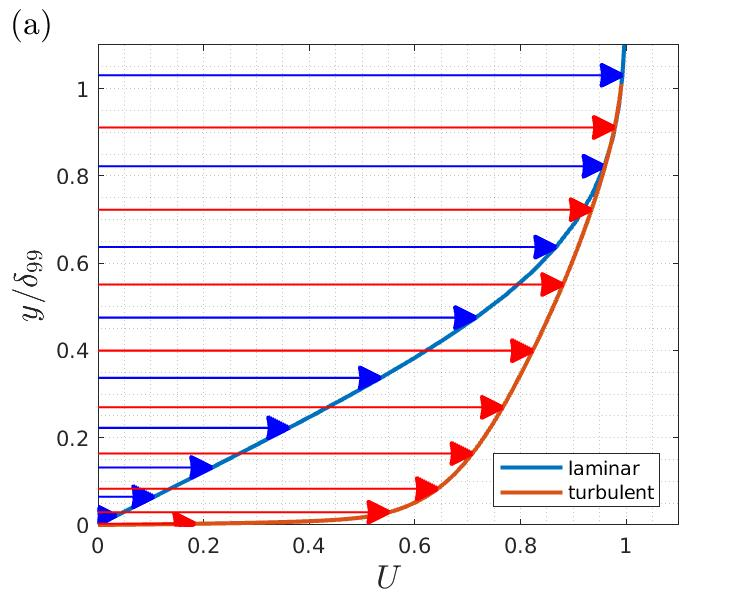
\includegraphics[width=0.5\textwidth]{ZPG_lam_turb.jpg}
\caption{ \label{fig:lam_turb_profiles} Mean streamwise velocity profile of a laminar (blue) and a turbulent ZPG (red) boundary layers.
   }
\end{figure}

In the case of curved boundaries, the curvature induces a pressure-gradient since the incoming flow has to adapt to the curvature of the wall. In a flat plate, a pressure-gradient can be produced by controlling the exterior flow, usually the streamwise gradient of the streamwise velocity $\pdv{U_{\infty}}/{x}$


\subsection{Turbulent boundary layers}
The characteristics of a boundary layer changes radically depending on the laminar/turbulent regime.
In a laminar boundary layer, any perturbation produces shear stresses and therefore, viscous forces, which are transported by the momentum of the flow and eventually dissipated by the viscous dissipation. 
High energetic perturbations, flow configurations or certain viscosity/momentum forces ratios are unstable, implying a change of regime, usually from the laminar regime to turbulence. 
The ratio between momentum and viscous forces is called Reynolds number $\Rey=U_{sc} L_{sc} / \nu$ and depending on the velocity scale $U_{sc}$ and the $L_{sc}$ chosen we would be analyzing different phenomena. The Reynolds number where a fluid configuration changes regime is called critical Reynolds number $\Rey_c$.
Other Reynolds number examples: if $U_{sc}=U_{\infty}$ and $L_{sc}=c$ where $c$ is the chord of a NACA profile, then we are setting the global configuration of the problem. If we want to analyze a local phenomena such as the different size of the fluid scales close to the wall compared to the largest ones inside the TBL, then we can use the Reynolds number based on the friction velocity $\Rey_{\tau}=u_{\tau}\delta_{99}/\nu$, where  $u_{\tau}(x)=\sqrt{(\tau_w / \rho)}$.

In the turbulent regime, the momentum and energy of the flow initiates a cascading effect breaking the initial ordered motions into chaotic submotions. 
Eddies are generated that extract energy from the mean flow and are divided into smaller eddies. Then a transport of energy between large and small eddies is produced. Eddies are regions with strong shear stresses, therefore the viscous forces are stronger and produce a dissipation of the kinetic energy.
The boundary layers studied here are momentum boundary layers that confine the turbulent perturbations and mayor viscous effects produced because of the presence of a solid boundary.

In a turbulent boundary layer, the thickness of the boundary layer should capture both the effects of the viscous forces as well as the turbulent fluctuations produced because of the presence of a solid boundary, leading to different definitions for the boundary layer thickness.

For laminar BLs and ZPG TBLs, the previous $\delta_{99}$ thickness, where the mean velocity of the flow is $99\%$ of the exterior velocity, is valid and is based only on the adaptation of the mean streamwise velocity to that of the outer flow.

For other TBLs with pressure gradients, the outer velocity can have gradients in the streamwise and wall-normal directions even without the presence of turbulence. In this case we can use an approach based on the level of turbulence such as the one used in \cite{diagnostic_Vinuesa} where the boundary layer thickness is such that it captures the turbulence up to certain turbulent level.
This approach is useful for the dataset that we use, since the turbulent levels outside of the TBL are minimal, both in the simulations \citep{E-AmorZPG, bobke2017, Pozuelo_JFM_22}, as in the experimental databases \citep{Sanmiguel_PRF}.
If the outer flow turbulent level is high, the method in \cite{diagnostic_Vinuesa} is not applicable. 
Other methods have been proposed in the literature and a review was given in \cite{d99_determination_2020}.

Turbulence presents a wide range of motions, the way we have been able to study and characterize turbulence is through decomposition of those characteristics. 
The first approach is an statistical characterization where we can divide the fluid variables into a mean or average value and a perturbation, this is known as the Reynolds decomposition \citep{Rey_decomp}.
The fluctuating character of the flow is shown for a flat plate APG TBL in Fig.~\ref{fig:lam_turb_development} where we show contour levels in snapshots of the instantaneous streamwise velocity. The contours in Fig.~\ref{fig:lam_turb_development}(a) are smooth and show a well-defined laminar behaviour with small perturbations introduced to trigger turbulence. In Fig.~\ref{fig:lam_turb_development}(b) the turbulence is totally developed It can be seen how at different streamwise positions $x/\delta^*_0$ the outer velocity or "edge velocity" $U_e$ decreases along $x$ to obtain an APG. The edge velocity is the velocity of the TBL at $y=\delta_{99}$ and depends on the method used to determine the boundary layer thickness.

\begin{figure}[h!]
\centering
% \captionsetup{width=0.99 \textwidth}
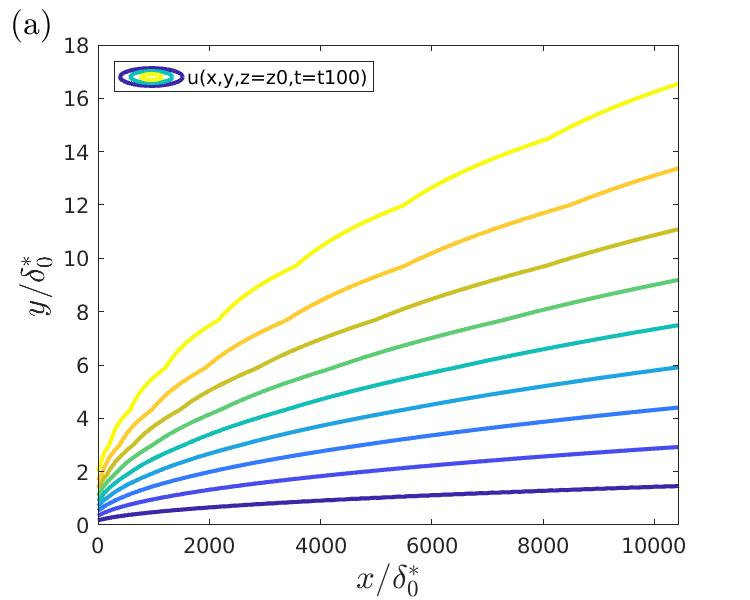
\includegraphics[width=0.49\textwidth ]{APG_laminar.jpg}
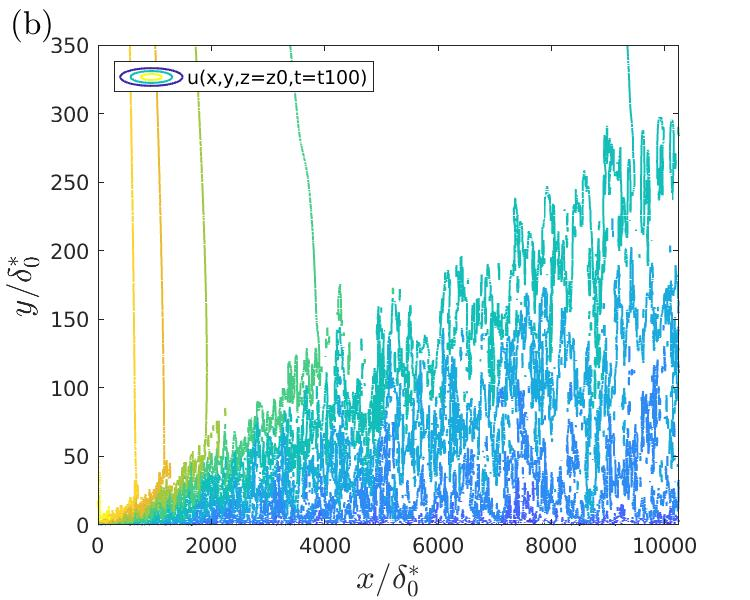
\includegraphics[width=0.49\textwidth]{APG_turb.jpg}
\caption{ \label{fig:lam_turb_development} Snapshot of the streamwise velocity $u(\vec(x), t)$ in a laminar (a) and a turbulent APG (b), boundary layers.
   }
\end{figure}



\section{Mathemathical analysis}

For an incompressible flow the conservation of mass in a control volume becomes the differential continuity equation (Eq.~\ref{eq:continuity_cap2}),

% Continuity
\begin{equation}
\label{eq:continuity_cap2}
% \overrightarrow{u}
    \nabla \cdot \vec{u} = \partial_i u_i = 
    \frac{\partial u}{\partial x} + \frac{\partial v}{\partial y} + \frac{\partial w}{\partial z} = 0,
\end{equation}
which is shown as the divergence of the velocity vector, the diadic and components notations.

To describe the time evolution of the fluid variables, the partial differential equations in Eq.~\ref{eq:NS_cap2} are the Navier--Stokes (NS) equations that describes the evolution of the momentum of the fluid as a function of the pressure gradient and viscous forces acting on it. The system of equations composed by Eqs.~\ref{eq:continuity_cap2} and \ref{eq:NS_cap2} are able to give both laminar and turbulent flow regimes, depending on the configuration of the problem.

% NS Total velocities
\begin{equation}
    \label{eq:NS_cap2}
    \frac {\partial u_i} {\partial t}  + u_j \frac {\partial u_i} {\partial x_j} =
    \frac {-1} {\rho} \frac {\partial p} {\partial x_i} +  \nu \frac {\partial^2 u_i} {\partial x_j^2}.
\end{equation}

By giving the correct scenario which is the boundary conditions (BCs) composed by an inflow, outflow, outer flow and wall-boundary conditions, together with an initial state of the system, we can expect either laminar flow or the change into a turbulent flow.



Once turbulence is fully-developed, the statistical approach to turbulence is based on the Reynolds decomposition \citep{Rey_decomp}, given in Eq.~\ref{eq:Rey_decomp}. This decomposition is based on a constant or averaged component and a fluctuating component in a way that once they are inputted into Eqs.~\ref{eq:continuity_cap2} and \ref{eq:NS_cap2} some of the partial differentials are simplified. An example is to use a constant base flow (such as the laminar state) plus a fluctuating flow field, this is the case used to study transition and stability of BLs. 
For our case, the mean flow $U_i$ is an average in time and the homogeneous directions. The average in a dimension $d$ is marked as $\langle . \rangle_d$, and the average in time and all the homogeneous dimensions is marked with $\overline{(.)}$. The mean velocity is $U_i = \overline{u_i} =\langle \langle u_i \rangle_z \rangle_t$ and as a result of Eq.~\ref{eq:Rey_decomp}, $\overline{u_i\myprime}=0$. Note that $\langle u_i\myprime \rangle_z (t) \neq 0$ and $\langle u_i\myprime \rangle_t(z) \neq 0$. 

Introducing the flow decomposition (Eq.~\ref{eq:Rey_decomp}) into the continuity and NS equations (Eqs.~\ref{eq:continuity_cap2} $\&$ \ref{eq:NS_cap2}), and using the total average in time and $z$, we see that the continuity equation is fulfilled for both the mean and the fluctuating component separately (Eq.~.\ref{eq:cont_decomp}). And in the NS equation we obtain the Reynolds Averaged Navier--Stokes equation (RANS) in Eq.~\ref{eq:RANS_cap2} and the equation for the time evolution of the perturbations Eq.~\ref{eq:pertub_cap2} as a result of substracting the RANS equations from the general NS equations.

% R Decomposition
\begin{equation}
    \label{eq:Rey_decomp}
    u_i = U_i + u_i\myprime.
\end{equation}

\begin{equation}
    \label{eq:cont_decomp}
    \partial_i \overline{u_i} = \partial_i \overline{U_i} = 0 ~~~~
    \partial_i \overline{U_i} + \partial_i \overline{u_i\myprime} = 0.  
\end{equation}

% RANS
\begin{equation}
    \label{eq:RANS_cap2}
    U_k\pdv{U_i}{x_k} + \pdv{\overline{u_i\myprime u_k\myprime}}{x_k} = \frac {-1} {\rho} \frac {\partial P}{\partial x_i} + \nu  \frac {\partial^2 U_k} {\partial x_k^2}.
\end{equation}

% Perturbations
\begin{equation}
    \label{eq:pertub_cap2}
    {\pdv{u_i\myprime}{t} + 
    U_k\pdv{u_i\myprime}{x_k} + u_k\myprime\pdv{u_i}{x_k} - \pdv{\overline{u_i\myprime u_k\myprime}}{x_k}  =
    \frac {-1} {\rho} \pdv{p\myprime}{x_i} + \nu  \frac {\partial^2 u_k\myprime} {\partial x_k^2}    }.
\end{equation}

Note that the RANS equation are similar to the NS equation, except that for the time derivative which is zero and an aditional term $\pdv{\overline{u_i\myprime u_k\myprime}}/{x_k}$ which can be included within the divergence of the viscous forces term, for that reason the terms $\rho \overline{u_i\myprime u_k\myprime}$ are called Reynolds-stresses. In the following, since the density is considered as constant, we will refer as Reynolds-stress (RS) to the terms in the tensor $\overline{u_i\myprime u_k\myprime}$, wich are also known as the variance or covariance of the total velocities $u_i$, $u_k$.
From the RANS equations it is interesting to see the mean velocities and the RS terms since they are an indicative of the level of turbulence and how it is affected by the pressure gradients and viscous forces on the right hand side (RHS) of the equation.

The equation for the perturbation velocities is useful since we can multiply by another perturbation velocity such as $u_{j}\myprime \cdot \left( \pdv{u_{i}\myprime}{t} + ... \right) $ or obtain the two-point correlation $\mathcal{R}_{u_i\myprime u_j\myprime}$ through the correlation denoted with the symbol $(\cdot \star \cdot)$ as in $ u_{i}\myprime \star \left( \pdv{u_{j}\myprime}{t} + ... \right)$. The former gives the Reynolds-stress transport equations (Eq.~\ref{eq:RS_transport_cap2}) where the turbulent kinetic energy budgets are a special case. The latter is used as in \cite{lee_moser_2019}, to obtain the power spectral density of each term of the Reynolds-stress transport equations.

Denoting Eq.~\ref{eq:NS_cap2} as $\mathrm{TOT}_i$, Eq.~\ref{eq:RANS_cap2} as $\mathrm{RANS}_i$ and Eq.~\ref{eq:RS_transport_cap2} as $\mathrm{PERT}_i$, the evolution equation for the total kinetic energy of the flow can be obtained through the multiplication,
% $\mathrm{KE} = (1/2) \overline{u_i \cdot \mathrm{TOT}_i}$, 
\begin{equation}
    \mathrm{KE} = (1/2) \overline{u_i \cdot \mathrm{TOT}_i}, 
\end{equation}
while the mean kinetic energy equation can be obtained with 
% $\mathrm{MKE} = (1/2) U_i \cdot \mathrm{RANS}_i$,
\begin{equation}
    \mathrm{MKE} = (1/2) U_i \cdot \mathrm{RANS}_i,
\end{equation}
and the turbulent kinetic energy equation with 
% $\mathrm{TKE} = (1/2) \overline{u_i\myprime \cdot \mathrm{PERT}_i} = KE - MKE$.
\begin{equation}
    \mathrm{TKE} = (1/2) \overline{u_i\myprime \cdot \mathrm{PERT}_i} = KE - MKE.
\end{equation}
In a similar way the Reynolds-stress transport ($RST_{ij}$) equation Eq.~\ref{eq:RS_transport_cap2} can be obtained by doing 
% $\mathrm{RS}_{ij} = \overline{u_i\myprime \cdot \mathrm{PERT_j} + u_j\myprime \cdot \mathrm{PERT_i}} $
\begin{multline}
    \mathrm{RST}_{ij} = \overline{u_i\myprime \cdot \mathrm{PERT_j} + u_j\myprime \cdot \mathrm{PERT_i}} = \\
    = \overline{u_i \cdot \mathrm{TOT_j} + u_j \cdot \mathrm{TOT_i}} - (U_i \cdot \mathrm{RANS}_j + U_j \cdot \mathrm{RANS}_i ) .
\end{multline}
% $\mathrm{RS}_{ij} = \overline{u_i \cdot \mathrm{TOT_j} + u_j \cdot \mathrm{TOT_i}} - (U_i \cdot \mathrm{RANS}_j + U_j \cdot \mathrm{RANS}_i )$.
% \begin{equation}
%     \mathrm{RS}_{ij} = \overline{u_i \cdot \mathrm{TOT_j} + u_j \cdot \mathrm{TOT_i}} - (U_i \cdot \mathrm{RANS}_j + U_j \cdot \mathrm{RANS}_i ) .
% \end{equation}

% RS transport equation
\begin{multline}
    \label{eq:RS_transport_cap2}
    \pdv{\overline{u_i\myprime u_j\myprime}}{t} + 
    U_k\pdv{\overline{u_i\myprime u_j\myprime}}{x_k} + 
    \left(
    \overline{u_i\myprime u_k\myprime}\pdv{U_j}{x_k} + \overline{u_j\myprime u_k\myprime}\pdv{U_i}{x_k}
    \right) +
    \left(
    \overline{u_i\myprime \pdv{u_j\myprime}{x_k} u_k\myprime} + \overline{\pdv{u_i\myprime}{x_k} u_j\myprime u_k\myprime}
    \right)
    = \\ 
    - \left( \overline{
    u_j\myprime \pdv{p\myprime}{x_i} + u_i\myprime \pdv{p\myprime}{x_j}
    } \right) 
    + \nu \frac{\partial^2 \overline{u_i\myprime u_j\myprime}}{\partial x_k^2} 
    - 2\nu \overline{\pdv{u_i\myprime}{x_k} \pdv{u_j\myprime}{x_k}}
\end{multline}

The third term in Eq.~\ref{eq:RS_transport_cap2} is specially interesting, after some manipulation, that term appears in the transport of $U_iU_j$ and the transport of $\overline{u_i\myprime u_j\myprime}$ with different signs. Usually is written on the right hand side of the equation and is called ``Production" since it substract energy from the mean flow and adds into the perturbations.
The other terms are presented in Appendix B from \textbf{Paper 1}.

